\documentclass[11pt,a4paper]{article}

\usepackage[utf8]{inputenc}
\usepackage[T1]{fontenc}
\usepackage[spanish]{babel}
\usepackage[margin=2.5cm]{geometry}
\usepackage{graphicx}
\usepackage{pdflscape}
\usepackage{listings}
\usepackage{xcolor}
\usepackage{longtable}
\usepackage{array}
\usepackage{booktabs}
\usepackage{hyperref}
\usepackage{fancyhdr}
\usepackage{enumitem}

\hypersetup{
    colorlinks=true,
    linkcolor=blue!50!black,
    urlcolor=blue!50!black,
    pdftitle={SGISI - Informe Tecnico},
}

\pagestyle{fancy}
\fancyhf{}
\fancyhead[L]{SGISI - Sistema de Gestion de Incidentes de Seguridad Informatica}
\fancyhead[R]{\thepage}
\renewcommand{\headrulewidth}{0.4pt}

% ───────────────────────── Estilos de codigo ─────────────────────────
\definecolor{codebg}{RGB}{247,249,251}
\definecolor{codekeyword}{RGB}{0,90,150}
\definecolor{codecomment}{RGB}{120,120,120}
\definecolor{codestring}{RGB}{160,40,40}

\lstdefinestyle{sqlstyle}{
    language=SQL,
    basicstyle=\ttfamily\scriptsize,
    keywordstyle=\color{codekeyword}\bfseries,
    commentstyle=\color{codecomment}\itshape,
    stringstyle=\color{codestring},
    numbers=left,
    numberstyle=\tiny\color{gray},
    numbersep=6pt,
    breaklines=true,
    breakatwhitespace=false,
    frame=single,
    rulecolor=\color{gray!40},
    backgroundcolor=\color{codebg},
    showstringspaces=false,
    tabsize=2,
    columns=flexible,
    upquote=true
}

\lstdefinestyle{codestyle}{
    basicstyle=\ttfamily\scriptsize,
    commentstyle=\color{codecomment}\itshape,
    numbers=left,
    numberstyle=\tiny\color{gray},
    numbersep=6pt,
    breaklines=true,
    breakatwhitespace=false,
    frame=single,
    rulecolor=\color{gray!40},
    backgroundcolor=\color{codebg},
    showstringspaces=false,
    tabsize=2,
    columns=flexible,
    upquote=true
}

\lstset{style=sqlstyle}

\newcommand{\codigo}[1]{\lstinline{#1}}

\begin{document}

% ════════════════════════════════════════════════════════════════
% CARATULA
% ════════════════════════════════════════════════════════════════
\begin{titlepage}
    \centering
    
\includegraphics[width=3.2cm]{images/logo_uni.png}\\[0.8cm]
    {\large\bfseries UNIVERSIDAD NACIONAL DE INGENIERÍA\\[2pt]}
    {\normalsize FACULTAD DE INGENIERÍA ELÉCTRICA Y ELECTRÓNICA\\[2pt]}
    {\normalsize Escuela de Ingeniería en Ciberseguridad\\}

    \vspace{2.5cm}
    {\Huge\bfseries SGISI\par}
    \vspace{0.4cm}
    {\Large Sistema de Gestión de Incidentes de\\ Seguridad Informática\par}

    \vspace{1.5cm}
    {\large\itshape Informe Técnico del Proyecto\par}

    \vspace{2.5cm}
    \begin{tabular}{rl}
        \textbf{Curso:}      & Base de Datos I (CBS04M) \\[4pt]
        \textbf{Docente:}    & Carpio Farfán, Pedro Manuel \\[4pt]
        \textbf{Integrantes:} & Borja Soto, Diego \\
                              & Escajadillo Gaspar, José \\
                              & Valencia Casanova, Fabrizio \\
    \end{tabular}

    \vfill
    {\large Lima, Perú -- 2026\par}
\end{titlepage}

\tableofcontents
\newpage

% ════════════════════════════════════════════════════════════════
% 1. JUSTIFICACION
% ════════════════════════════════════════════════════════════════
\section{Justificación}

Una empresa peruana de consultoría en ciberseguridad brinda servicios de monitoreo y
respuesta a varias organizaciones. Debido a que anteriormente la información se
registraba en hojas de cálculo compartidas, se generaban problemas de pérdida de
información, duplicidad de registros y falta de trazabilidad sobre los incidentes
detectados y los activos comprometidos.

Por ello, se desarrolló un \textbf{Sistema de Gestión de Incidentes de Seguridad
Informática (SGISI)} que permite almacenar de manera centralizada la información de
las organizaciones, registrando para cada una un identificador único, el nombre del
departamento responsable, el responsable del área y la cantidad de activos
administrados. Cada organización puede contar con varios analistas de seguridad y
administrar múltiples activos tecnológicos, mientras que cada analista y cada activo
pertenecen a una única organización.

De los analistas se almacena un identificador, nombre, apellido, cargo,
especialización, nivel de acceso, correo electrónico y teléfono; mientras que de los
activos se registra un identificador, nombre, dirección IP, sistema operativo y nivel
de criticidad. Adicionalmente, los analistas se clasifican en dos tipos: Supervisores
y Supervisados. Un analista supervisor puede supervisar a varios analistas
supervisados, mientras que cada analista supervisado depende de un único supervisor;
del supervisor se registra el número de analistas a su cargo, y del supervisado su
nivel de experiencia y el área en la que opera. Un analista solo puede pertenecer a
uno de estos tipos, por lo que no puede ser supervisor y supervisado al mismo tiempo.

Los activos pueden presentar diversas vulnerabilidades de seguridad, registrándose
para cada una un identificador, código CVE, descripción, severidad CVSS, fecha de
descubrimiento y estado. Los analistas son responsables de gestionar los incidentes de
seguridad: un analista puede atender varios incidentes, mientras que cada incidente
tiene un único analista responsable. Los activos generan alertas de seguridad; varias
alertas pueden escalar a un mismo incidente, aunque una alerta puede no estar asociada
a ninguno. Un incidente puede afectar a varios activos y un mismo activo puede verse
comprometido en distintos incidentes, registrándose para cada asociación el impacto
ocasionado y la fecha de detección. Finalmente, los incidentes pueden generar uno o
varios reportes, elaborados por un analista.

Con el fin de garantizar la trazabilidad de las operaciones efectuadas sobre los
incidentes, el sistema mantiene además una \textbf{bitácora de auditoría} que conserva
el historial de todos los cambios realizados sobre ellos, asociada al analista
responsable del incidente auditado.

% ════════════════════════════════════════════════════════════════
% 2. DIAGRAMA
% ════════════════════════════════════════════════════════════════
\section{Diagrama}

\begin{landscape}
\begin{figure}[p]
    \centering
    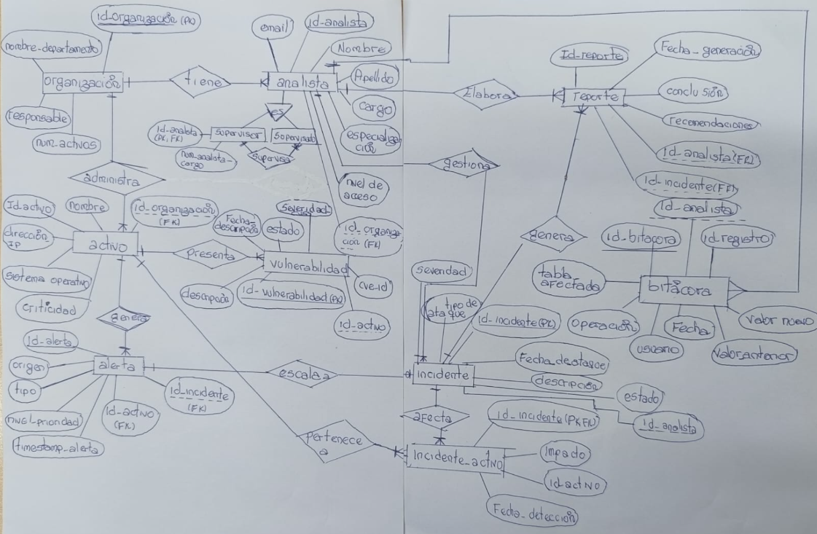
\includegraphics[width=\linewidth]{images/diagrama_er.png}
    \caption{Diagrama entidad-relación de SGISI.}
\end{figure}
\end{landscape}

% ════════════════════════════════════════════════════════════════
% 3. ESQUEMA LOGICO
% ════════════════════════════════════════════════════════════════
\section{Esquema lógico}

A continuación se presenta el esquema lógico relacional de SGISI: cada entidad se
expresa como \texttt{TABLA(atributos)}, indicando su clave primaria (PK) y sus claves
foráneas (FK).

\begin{description}[leftmargin=0pt, style=nextline]

\item[\texttt{ORGANIZACION(id\_organizacion, nombre\_departamento, responsable, num\_activos)}]
PK = id\_organizacion

\item[\texttt{ANALISTA(id\_analista, nombre, apellido, cargo, especializacion, nivel\_acceso, email, telefono, id\_organizacion)}]
PK = id\_analista \\
FK = id\_organizacion de ORGANIZACION

\item[\texttt{SUPERVISOR(id\_analista, num\_analistas\_cargo)}]
PK = id\_analista \\
FK = id\_analista de ANALISTA

\item[\texttt{SUPERVISADO(id\_analista, nivel\_experiencia, area\_operacion)}]
PK = id\_analista \\
FK = id\_analista de ANALISTA

\item[\texttt{ACTIVO(id\_activo, nombre, direccion\_ip, sistema\_operativo, criticidad, id\_organizacion)}]
PK = id\_activo \\
FK = id\_organizacion de ORGANIZACION

\item[\texttt{VULNERABILIDAD(id\_vulnerabilidad, cve\_id, descripcion, severidad\_cvss, fecha\_descubrimiento, estado, id\_activo)}]
PK = id\_vulnerabilidad \\
FK = id\_activo de ACTIVO

\item[\texttt{INCIDENTE(id\_incidente, tipo\_ataque, fecha\_hora, descripcion, estado, severidad, id\_analista)}]
PK = id\_incidente \\
FK = id\_analista de ANALISTA

\item[\texttt{ALERTA(id\_alerta, origen, timestamp\_alerta, tipo, nivel\_prioridad, id\_activo, id\_incidente)}]
PK = id\_alerta \\
FK = id\_activo de ACTIVO \\
FK = id\_incidente de INCIDENTE (opcional)

\item[\texttt{INCIDENTE\_ACTIVO(id\_incidente, id\_activo, impacto, fecha\_deteccion)}]
PK = (id\_incidente, id\_activo) \\
FK = id\_incidente de INCIDENTE \\
FK = id\_activo de ACTIVO

\item[\texttt{REPORTE(id\_reporte, fecha\_generacion, conclusiones, recomendaciones, id\_analista, id\_incidente)}]
PK = id\_reporte \\
FK = id\_analista de ANALISTA \\
FK = id\_incidente de INCIDENTE

\item[\texttt{BITACORA(id\_bitacora, tabla\_afectada, operacion, id\_registro, usuario, fecha, valor\_anterior, valor\_nuevo, id\_analista)}]
PK = id\_bitacora \\
FK = id\_analista de ANALISTA \\
\textit{(id\_registro NO es FK a INCIDENTE de forma deliberada, para no perder el
rastro de auditoría si el incidente llegara a eliminarse.)}

\end{description}

% ════════════════════════════════════════════════════════════════
% 4. ESQUEMA FISICO
% ════════════════════════════════════════════════════════════════
\section{Esquema físico}

Se presenta a continuación el código T-SQL de creación de las 11 tablas de SGISI,
con sus atributos, tipos de datos y restricciones (claves primarias, claves foráneas,
\texttt{CHECK}, \texttt{DEFAULT} y \texttt{UNIQUE}).

\begin{lstlisting}
CREATE DATABASE SGISI;
GO
USE SGISI;
GO

CREATE TABLE ORGANIZACION (
    id_organizacion     INT IDENTITY(1,1) PRIMARY KEY,
    nombre_departamento VARCHAR(100) NOT NULL,
    responsable         VARCHAR(100) NOT NULL,
    num_activos         INT NULL DEFAULT (0)
                        CHECK (num_activos >= 0)
);
GO

CREATE TABLE ANALISTA (
    id_analista      INT IDENTITY(1,1) PRIMARY KEY,
    nombre           VARCHAR(80)  NOT NULL,
    apellido         VARCHAR(80)  NOT NULL,
    cargo            VARCHAR(100) NOT NULL,
    especializacion  VARCHAR(100) NULL,
    nivel_acceso     TINYINT NOT NULL
                     CHECK (nivel_acceso >= 1 AND nivel_acceso <= 5),
    email            VARCHAR(150) NOT NULL UNIQUE,
    telefono         VARCHAR(20)  NULL,
    id_organizacion  INT NOT NULL,
    CONSTRAINT FK_ANALISTA_ORG FOREIGN KEY (id_organizacion)
        REFERENCES ORGANIZACION(id_organizacion) ON DELETE CASCADE
);
GO

CREATE TABLE SUPERVISOR (
    id_analista          INT PRIMARY KEY,
    num_analistas_cargo  INT NULL DEFAULT (0)
                         CHECK (num_analistas_cargo >= 0),
    CONSTRAINT FK_SUPERVISOR_ANALISTA FOREIGN KEY (id_analista)
        REFERENCES ANALISTA(id_analista) ON DELETE CASCADE
);
GO

CREATE TABLE SUPERVISADO (
    id_analista       INT PRIMARY KEY,
    nivel_experiencia VARCHAR(20)  NOT NULL
                      CHECK (nivel_experiencia IN ('Senior','Mid','Junior')),
    area_operacion    VARCHAR(100) NOT NULL,
    CONSTRAINT FK_SUPERVISADO_ANALISTA FOREIGN KEY (id_analista)
        REFERENCES ANALISTA(id_analista) ON DELETE CASCADE
);
GO

CREATE TABLE ACTIVO (
    id_activo          INT IDENTITY(1,1) PRIMARY KEY,
    nombre             VARCHAR(100) NOT NULL,
    direccion_ip       VARCHAR(45) NULL,
    sistema_operativo  VARCHAR(80) NULL,
    criticidad         VARCHAR(10) NOT NULL
                       CHECK (criticidad IN ('CRITICA','ALTA','MEDIA','BAJA')),
    id_organizacion    INT NOT NULL,
    CONSTRAINT FK_ACTIVO_ORG FOREIGN KEY (id_organizacion)
        REFERENCES ORGANIZACION(id_organizacion)
);
GO

CREATE TABLE VULNERABILIDAD (
    id_vulnerabilidad     INT IDENTITY(1,1) PRIMARY KEY,
    cve_id                VARCHAR(30) NULL UNIQUE,
    descripcion           VARCHAR(500) NOT NULL,
    severidad_cvss        DECIMAL(3,1) NULL
                          CHECK (severidad_cvss >= 0.0 AND severidad_cvss <= 10.0),
    fecha_descubrimiento  DATE NOT NULL DEFAULT (GETDATE()),
    estado                VARCHAR(20) NOT NULL
                          CHECK (estado IN ('PARCHEADA','EN_PROCESO','PENDIENTE')),
    id_activo             INT NOT NULL,
    CONSTRAINT FK_VULN_ACTIVO FOREIGN KEY (id_activo)
        REFERENCES ACTIVO(id_activo) ON DELETE CASCADE
);
GO

CREATE TABLE INCIDENTE (
    id_incidente  INT IDENTITY(1,1) PRIMARY KEY,
    tipo_ataque   VARCHAR(100) NOT NULL,
    fecha_hora    DATETIME NOT NULL DEFAULT (GETDATE()),
    descripcion   VARCHAR(1000) NULL,
    estado        VARCHAR(20) NOT NULL
                  CHECK (estado IN ('ABIERTO','EN_INVESTIGACION','CERRADO')),
    severidad     DECIMAL(3,1) NULL
                  CHECK (severidad >= 0.0 AND severidad <= 10.0),
    id_analista   INT NOT NULL,
    CONSTRAINT FK_INCIDENTE_ANALISTA FOREIGN KEY (id_analista)
        REFERENCES ANALISTA(id_analista)
);
GO

CREATE TABLE ALERTA (
    id_alerta         INT IDENTITY(1,1) PRIMARY KEY,
    origen            VARCHAR(50) NOT NULL
                      CHECK (origen IN ('MANUAL','ANTIVIRUS','FIREWALL','SIEM','IDS')),
    timestamp_alerta  DATETIME NOT NULL DEFAULT (GETDATE()),
    tipo              VARCHAR(100) NOT NULL,
    nivel_prioridad   VARCHAR(10) NOT NULL
                      CHECK (nivel_prioridad IN ('CRITICA','ALTA','MEDIA','BAJA')),
    id_activo         INT NOT NULL,
    id_incidente      INT NULL,
    CONSTRAINT FK_ALERTA_ACTIVO FOREIGN KEY (id_activo)
        REFERENCES ACTIVO(id_activo) ON DELETE CASCADE,
    CONSTRAINT FK_ALERTA_INCIDENTE FOREIGN KEY (id_incidente)
        REFERENCES INCIDENTE(id_incidente)
);
GO

CREATE TABLE INCIDENTE_ACTIVO (
    id_incidente     INT NOT NULL,
    id_activo        INT NOT NULL,
    impacto          VARCHAR(20) NULL
                     CHECK (impacto IN ('CRITICO','GRAVE','MODERADO','LEVE')),
    fecha_deteccion  DATETIME NULL DEFAULT (GETDATE()),
    CONSTRAINT PK_INCIDENTE_ACTIVO PRIMARY KEY (id_incidente, id_activo),
    CONSTRAINT FK_IA_INCIDENTE FOREIGN KEY (id_incidente)
        REFERENCES INCIDENTE(id_incidente) ON DELETE CASCADE,
    CONSTRAINT FK_IA_ACTIVO FOREIGN KEY (id_activo)
        REFERENCES ACTIVO(id_activo) ON DELETE CASCADE
);
GO

CREATE TABLE REPORTE (
    id_reporte        INT IDENTITY(1,1) PRIMARY KEY,
    fecha_generacion  DATE NOT NULL DEFAULT (GETDATE()),
    conclusiones      VARCHAR(2000) NULL,
    recomendaciones   VARCHAR(2000) NULL,
    id_analista       INT NOT NULL,
    id_incidente      INT NOT NULL,
    CONSTRAINT FK_REPORTE_ANALISTA FOREIGN KEY (id_analista)
        REFERENCES ANALISTA(id_analista),
    CONSTRAINT FK_REPORTE_INCIDENTE FOREIGN KEY (id_incidente)
        REFERENCES INCIDENTE(id_incidente) ON DELETE CASCADE
);
GO

-- Entidad de auditoria: registra los cambios sobre INCIDENTE
CREATE TABLE BITACORA (
    id_bitacora     INT IDENTITY(1,1) PRIMARY KEY,
    tabla_afectada  VARCHAR(100) NOT NULL,
    operacion       VARCHAR(10) NOT NULL
                    CHECK (operacion IN ('INSERT','UPDATE','DELETE')),
    id_registro     INT NULL,
    usuario         SYSNAME NOT NULL DEFAULT (SUSER_SNAME()),
    fecha           DATETIME NOT NULL DEFAULT (GETDATE()),
    valor_anterior  VARCHAR(MAX) NULL,
    valor_nuevo     VARCHAR(MAX) NULL,
    id_analista     INT NULL,
    CONSTRAINT FK_BITACORA_ANALISTA FOREIGN KEY (id_analista)
        REFERENCES ANALISTA(id_analista)
);
GO
\end{lstlisting}

% ════════════════════════════════════════════════════════════════
% 5. PROGRAMAS
% ════════════════════════════════════════════════════════════════
\section{Programas}

Además de las estructuras estáticas de datos, SGISI implementa lógica de negocio
directamente en el motor de la base de datos mediante cuatro tipos de objetos
programables: funciones, procedimientos almacenados, triggers y un cursor.

\subsection{Funciones}

Una \textbf{función} es un objeto que recibe parámetros y devuelve un valor escalar
o una tabla; se invoca dentro de consultas y \emph{no modifica} los datos. SGISI
utiliza diez funciones:

\begin{description}[leftmargin=0pt, style=nextline]
\item[\texttt{fn\_BuscarOrganizacion}] Busca una organización por su identificador.
\item[\texttt{fn\_BuscarAnalista}] Busca un analista por su identificador.
\item[\texttt{fn\_BuscarIncidente}] Busca incidentes por identificador o por
coincidencia parcial en el tipo de ataque.
\item[\texttt{fn\_BuscarAlerta}] Busca alertas por identificador o por coincidencia
parcial en el tipo.
\item[\texttt{fn\_BuscarReporte}] Busca reportes por identificador o por coincidencia
parcial en las conclusiones.
\item[\texttt{fn\_BuscarVulnerabilidad}] Busca una vulnerabilidad por su
identificador.
\item[\texttt{fn\_HistorialIncidentesPorActivo}] Devuelve todos los incidentes que
han afectado a un activo específico, junto con el impacto ocasionado.
\item[\texttt{fn\_ListarActivosCriticos}] Lista los activos de criticidad ALTA o
CRÍTICA de una organización.
\item[\texttt{fn\_ContarIncidentesPorAnalista}] Devuelve cuántos incidentes tiene
asignados un analista.
\item[\texttt{fn\_SeveridadPromedioOrganizacion}] Calcula la severidad promedio de
los incidentes de una organización.
\end{description}

\begin{lstlisting}
CREATE FUNCTION fn_BuscarOrganizacion (@id INT = NULL, @nombre_depto VARCHAR(100) = NULL)
RETURNS TABLE AS RETURN
(
    SELECT id_organizacion, num_activos
    FROM dbo.ORGANIZACION
    WHERE (@id IS NOT NULL AND id_organizacion = @id)
)
GO

CREATE FUNCTION fn_BuscarAnalista (@id INT = NULL, @cargo VARCHAR(100) = NULL)
RETURNS TABLE AS RETURN
(
    SELECT id_analista, id_organizacion
    FROM dbo.ANALISTA
    WHERE (@id IS NOT NULL AND id_analista = @id)
)
GO

CREATE FUNCTION fn_BuscarIncidente (@id INT = NULL, @tipo_ataque VARCHAR(100) = NULL)
RETURNS TABLE AS RETURN
(
    SELECT id_incidente, tipo_ataque, fecha_hora, descripcion, estado, severidad, id_analista
    FROM dbo.INCIDENTE
    WHERE (@id IS NOT NULL AND id_incidente = @id)
       OR (@tipo_ataque IS NOT NULL AND tipo_ataque LIKE '%' + @tipo_ataque + '%')
);
GO

CREATE FUNCTION fn_BuscarAlerta (@id INT = NULL, @tipo VARCHAR(100) = NULL)
RETURNS TABLE AS RETURN
(
    SELECT id_alerta, origen, timestamp_alerta, tipo, nivel_prioridad, id_activo, id_incidente
    FROM dbo.ALERTA
    WHERE (@id IS NOT NULL AND id_alerta = @id)
       OR (@tipo IS NOT NULL AND tipo LIKE '%' + @tipo + '%')
);
GO

CREATE FUNCTION fn_BuscarReporte (@id INT = NULL, @conclusiones VARCHAR(2000) = NULL)
RETURNS TABLE AS RETURN
(
    SELECT id_reporte, fecha_generacion, conclusiones, recomendaciones, id_incidente, id_analista
    FROM dbo.REPORTE
    WHERE (@id IS NOT NULL AND id_reporte = @id)
       OR (@conclusiones IS NOT NULL AND conclusiones LIKE '%' + @conclusiones + '%')
);
GO

CREATE FUNCTION fn_BuscarVulnerabilidad (@id INT = NULL)
RETURNS TABLE AS RETURN
(
    SELECT id_vulnerabilidad, descripcion, estado
    FROM dbo.VULNERABILIDAD
    WHERE (@id IS NOT NULL AND id_vulnerabilidad = @id)
);
GO

CREATE FUNCTION fn_HistorialIncidentesPorActivo (@id_activo INT)
RETURNS TABLE
AS
RETURN
(
    SELECT
        IA.id_activo,
        I.id_incidente,
        I.tipo_ataque,
        I.estado AS estado_incidente,
        I.severidad AS severidad_incidente,
        IA.impacto,
        IA.fecha_deteccion
    FROM dbo.INCIDENTE_ACTIVO IA
    JOIN dbo.INCIDENTE I ON IA.id_incidente = I.id_incidente
    WHERE IA.id_activo = @id_activo
);
GO

CREATE FUNCTION fn_ListarActivosCriticos(@id_organizacion INT)
RETURNS TABLE
AS
RETURN
(
    SELECT id_activo, nombre, direccion_ip, sistema_operativo, criticidad
    FROM ACTIVO
    WHERE id_organizacion = @id_organizacion
      AND criticidad IN ('ALTA','CRITICA')
);
GO

CREATE FUNCTION fn_ContarIncidentesPorAnalista(@id_analista INT)
RETURNS INT
AS
BEGIN
    DECLARE @total INT;
    SELECT @total = COUNT(*)
    FROM INCIDENTE
    WHERE id_analista = @id_analista;
    RETURN @total;
END;
GO

CREATE FUNCTION fn_SeveridadPromedioOrganizacion(@id_organizacion INT)
RETURNS DECIMAL(5,2)
AS
BEGIN
    DECLARE @promedio DECIMAL(5,2);
    SELECT @promedio = AVG(I.severidad)
    FROM INCIDENTE I
    JOIN ANALISTA A ON I.id_analista = A.id_analista
    WHERE A.id_organizacion = @id_organizacion;
    RETURN ISNULL(@promedio, 0);
END;
GO
\end{lstlisting}

\subsection{Procedimientos almacenados}

Un \textbf{procedimiento almacenado} es un bloque de instrucciones que sí ejecuta
acciones sobre los datos (insertar, actualizar); en SGISI, cada uno de escritura se
protege con una \textbf{transacción} explícita (\texttt{BEGIN TRANSACTION} /
\texttt{COMMIT} / \texttt{ROLLBACK}) dentro de un bloque \texttt{TRY...CATCH}, de
modo que ante cualquier error toda la operación se deshace por completo. SGISI
utiliza seis procedimientos:

\begin{description}[leftmargin=0pt, style=nextline]
\item[\texttt{sp\_RegistrarIncidente}] Registra un nuevo incidente, asignándole la
fecha exacta y el estado inicial \texttt{ABIERTO}.
\item[\texttt{sp\_RegistrarAlerta}] Registra una alerta generada por un activo.
\item[\texttt{sp\_AsignarActivoAIncidente}] Vincula un activo a un incidente en la
tabla puente, validando que ambos existan.
\item[\texttt{sp\_CerrarIncidente}] Cambia el estado del incidente a \texttt{CERRADO}
y, en la misma transacción, registra el reporte con conclusiones y recomendaciones.
\item[\texttt{sp\_GenerarReporte}] Genera un reporte para un incidente existente.
\item[\texttt{sp\_ResumenSeguridadPorAnalista}] Procedimiento con \textbf{cursor}
(se explica en la sección~\ref{sec:cursor}).
\end{description}

\begin{lstlisting}
CREATE PROCEDURE sp_RegistrarIncidente
    @tipo_ataque VARCHAR(100),
    @descripcion VARCHAR(1000),
    @severidad   DECIMAL(3,1),
    @id_analista INT
AS
BEGIN
    SET NOCOUNT ON;
    BEGIN TRANSACTION;
    BEGIN TRY
        INSERT INTO INCIDENTE
            (tipo_ataque, fecha_hora, descripcion, estado, severidad, id_analista)
        VALUES
            (@tipo_ataque, GETDATE(), @descripcion, 'ABIERTO', @severidad, @id_analista);
        COMMIT TRANSACTION;
        SELECT SCOPE_IDENTITY() AS id_incidente_creado;
    END TRY
    BEGIN CATCH
        ROLLBACK TRANSACTION;
        THROW;
    END CATCH
END;
GO

CREATE PROCEDURE sp_RegistrarAlerta
    @origen         VARCHAR(50),
    @tipo           VARCHAR(100),
    @nivel_prioridad VARCHAR(10),
    @id_activo      INT,
    @id_incidente   INT = NULL
AS
BEGIN
    BEGIN TRANSACTION;
    BEGIN TRY
        INSERT INTO ALERTA
            (origen, timestamp_alerta, tipo, nivel_prioridad, id_activo, id_incidente)
        VALUES
            (@origen, GETDATE(), @tipo, @nivel_prioridad, @id_activo, @id_incidente);
        COMMIT TRANSACTION;
        SELECT SCOPE_IDENTITY() AS id_alerta_creada;
    END TRY
    BEGIN CATCH
        ROLLBACK TRANSACTION;
        THROW;
    END CATCH
END;
GO

CREATE PROCEDURE sp_AsignarActivoAIncidente
    @id_incidente INT,
    @id_activo    INT,
    @impacto      VARCHAR(20)
AS
BEGIN
    BEGIN TRANSACTION;
    BEGIN TRY
        IF NOT EXISTS (SELECT 1 FROM INCIDENTE WHERE id_incidente = @id_incidente)
            THROW 50001, 'El incidente especificado no existe.', 1;
        IF NOT EXISTS (SELECT 1 FROM ACTIVO WHERE id_activo = @id_activo)
            THROW 50002, 'El activo especificado no existe.', 1;
        INSERT INTO INCIDENTE_ACTIVO (id_incidente, id_activo, impacto, fecha_deteccion)
        VALUES (@id_incidente, @id_activo, @impacto, GETDATE());
        COMMIT TRANSACTION;
    END TRY
    BEGIN CATCH
        ROLLBACK TRANSACTION;
        THROW;
    END CATCH
END;
GO

CREATE PROCEDURE sp_CerrarIncidente
    @id_incidente INT,
    @conclusiones VARCHAR(2000),
    @recomendaciones VARCHAR(2000),
    @id_analista  INT
AS
BEGIN
    BEGIN TRANSACTION;
    BEGIN TRY
        UPDATE INCIDENTE
        SET estado = 'CERRADO'
        WHERE id_incidente = @id_incidente;

        INSERT INTO REPORTE
            (fecha_generacion, conclusiones, recomendaciones, id_analista, id_incidente)
        VALUES
            (GETDATE(), @conclusiones, @recomendaciones, @id_analista, @id_incidente);
        COMMIT TRANSACTION;
    END TRY
    BEGIN CATCH
        ROLLBACK TRANSACTION;
        THROW;
    END CATCH
END;
GO

CREATE PROCEDURE sp_GenerarReporte
    @id_incidente    INT,
    @conclusiones    VARCHAR(2000),
    @recomendaciones VARCHAR(2000),
    @id_analista     INT
AS
BEGIN
    BEGIN TRANSACTION;
    BEGIN TRY
        IF NOT EXISTS (SELECT 1 FROM INCIDENTE WHERE id_incidente = @id_incidente)
            THROW 50003, 'El incidente especificado no existe.', 1;
        INSERT INTO REPORTE
            (fecha_generacion, conclusiones, recomendaciones, id_analista, id_incidente)
        VALUES
            (GETDATE(), @conclusiones, @recomendaciones, @id_analista, @id_incidente);
        COMMIT TRANSACTION;
        SELECT SCOPE_IDENTITY() AS id_reporte_creado;
    END TRY
    BEGIN CATCH
        ROLLBACK TRANSACTION;
        THROW;
    END CATCH
END;
GO
\end{lstlisting}

\subsection{Triggers}

Un \textbf{trigger} (disparador) es un objeto que se ejecuta automáticamente como
reacción a un cambio en una tabla (\texttt{INSERT}, \texttt{UPDATE} o
\texttt{DELETE}), sin que ninguna aplicación lo invoque explícitamente. SGISI utiliza
seis triggers:

\begin{description}[leftmargin=0pt, style=nextline]
\item[\texttt{trg\_ActualizarNumActivos\_Insert}] Incrementa el contador de activos
de la organización cuando se agrega un activo.
\item[\texttt{trg\_ActualizarNumActivos\_Delete}] Decrementa el contador de activos
cuando se elimina un activo.
\item[\texttt{trg\_ActualizarNumActivos\_Update}] Ajusta los contadores de origen y
destino cuando un activo cambia de organización.
\item[\texttt{trg\_ValidarEspecializacionDisjunta}] Impide registrar como
\emph{Supervisado} a un analista que ya es \emph{Supervisor}.
\item[\texttt{trg\_ValidarSupervisorDisjunto}] Impide registrar como
\emph{Supervisor} a un analista que ya es \emph{Supervisado}.
\item[\texttt{trg\_AuditarIncidente}] Ante cualquier \texttt{INSERT}, \texttt{UPDATE}
o \texttt{DELETE} sobre \texttt{INCIDENTE}, registra el cambio en \texttt{BITACORA}
(usuario, fecha, valores anterior y nuevo), sin intervención de la aplicación.
\end{description}

\begin{lstlisting}
CREATE TRIGGER trg_ActualizarNumActivos_Insert
ON ACTIVO
AFTER INSERT
AS
BEGIN
    UPDATE ORGANIZACION
    SET num_activos = num_activos + 1
    WHERE id_organizacion IN (SELECT id_organizacion FROM inserted);
END;
GO

CREATE TRIGGER trg_ActualizarNumActivos_Delete
ON ACTIVO
AFTER DELETE
AS
BEGIN
    UPDATE ORGANIZACION
    SET num_activos = num_activos - 1
    WHERE id_organizacion IN (SELECT id_organizacion FROM deleted);
END;
GO

CREATE TRIGGER trg_ActualizarNumActivos_Update
ON dbo.ACTIVO
AFTER UPDATE
AS
BEGIN
    SET NOCOUNT ON;
    IF UPDATE(id_organizacion)
    BEGIN
        UPDATE o
        SET o.num_activos = o.num_activos - x.cnt
        FROM dbo.ORGANIZACION o
        JOIN (SELECT id_organizacion, COUNT(*) AS cnt
              FROM deleted GROUP BY id_organizacion) x
          ON o.id_organizacion = x.id_organizacion;

        UPDATE o
        SET o.num_activos = o.num_activos + x.cnt
        FROM dbo.ORGANIZACION o
        JOIN (SELECT id_organizacion, COUNT(*) AS cnt
              FROM inserted GROUP BY id_organizacion) x
          ON o.id_organizacion = x.id_organizacion;
    END
END;
GO

CREATE TRIGGER trg_ValidarEspecializacionDisjunta
ON SUPERVISADO
AFTER INSERT
AS
BEGIN
    IF EXISTS (
        SELECT 1 FROM inserted I
        JOIN SUPERVISOR S ON I.id_analista = S.id_analista
    )
    BEGIN
        ROLLBACK TRANSACTION;
        THROW 50010, 'Un analista no puede ser Supervisor y Supervisado al mismo tiempo.', 1;
    END
END;
GO

CREATE TRIGGER trg_ValidarSupervisorDisjunto
ON SUPERVISOR
AFTER INSERT
AS
BEGIN
    IF EXISTS (
        SELECT 1 FROM inserted I
        JOIN SUPERVISADO S ON I.id_analista = S.id_analista
    )
    BEGIN
        ROLLBACK TRANSACTION;
        THROW 50011, 'Un analista no puede ser Supervisado y Supervisor al mismo tiempo.', 1;
    END
END;
GO

CREATE TRIGGER trg_AuditarIncidente
ON dbo.INCIDENTE
AFTER INSERT, UPDATE, DELETE
AS
BEGIN
    SET NOCOUNT ON;
    DECLARE @hayIns BIT = CASE WHEN EXISTS(SELECT 1 FROM inserted) THEN 1 ELSE 0 END;
    DECLARE @hayDel BIT = CASE WHEN EXISTS(SELECT 1 FROM deleted)  THEN 1 ELSE 0 END;

    IF @hayIns = 1 AND @hayDel = 1
    BEGIN
        INSERT INTO dbo.BITACORA (tabla_afectada, operacion, id_registro, id_analista, valor_anterior, valor_nuevo)
        SELECT 'INCIDENTE', 'UPDATE', i.id_incidente, i.id_analista,
               'estado=' + ISNULL(d.estado COLLATE DATABASE_DEFAULT,'NULL')
                 + '; severidad=' + ISNULL(CAST(d.severidad AS VARCHAR(10)),'NULL')
                 + '; analista=' + ISNULL(CAST(d.id_analista AS VARCHAR(10)),'NULL'),
               'estado=' + ISNULL(i.estado COLLATE DATABASE_DEFAULT,'NULL')
                 + '; severidad=' + ISNULL(CAST(i.severidad AS VARCHAR(10)),'NULL')
                 + '; analista=' + ISNULL(CAST(i.id_analista AS VARCHAR(10)),'NULL')
        FROM inserted i JOIN deleted d ON i.id_incidente = d.id_incidente;
    END
    ELSE IF @hayIns = 1
    BEGIN
        INSERT INTO dbo.BITACORA (tabla_afectada, operacion, id_registro, id_analista, valor_anterior, valor_nuevo)
        SELECT 'INCIDENTE', 'INSERT', i.id_incidente, i.id_analista, NULL,
               'estado=' + ISNULL(i.estado COLLATE DATABASE_DEFAULT,'NULL')
                 + '; severidad=' + ISNULL(CAST(i.severidad AS VARCHAR(10)),'NULL')
                 + '; tipo=' + ISNULL(i.tipo_ataque COLLATE DATABASE_DEFAULT,'NULL')
        FROM inserted i;
    END
    ELSE IF @hayDel = 1
    BEGIN
        INSERT INTO dbo.BITACORA (tabla_afectada, operacion, id_registro, id_analista, valor_anterior, valor_nuevo)
        SELECT 'INCIDENTE', 'DELETE', d.id_incidente, d.id_analista,
               'estado=' + ISNULL(d.estado COLLATE DATABASE_DEFAULT,'NULL')
                 + '; severidad=' + ISNULL(CAST(d.severidad AS VARCHAR(10)),'NULL')
                 + '; tipo=' + ISNULL(d.tipo_ataque COLLATE DATABASE_DEFAULT,'NULL'),
               NULL
        FROM deleted d;
    END
END;
GO
\end{lstlisting}

\subsection{Cursor}
\label{sec:cursor}

Un \textbf{cursor} permite recorrer un resultado \emph{fila por fila} de manera
secuencial, a diferencia de las operaciones habituales que procesan un conjunto
completo de registros a la vez. En SGISI, el procedimiento
\texttt{sp\_ResumenSeguridadPorAnalista} utiliza un cursor para recorrer, uno por
uno, a todos los analistas registrados y, para cada uno, invoca las funciones
\texttt{fn\_ContarIncidentesPorAnalista} y \texttt{fn\_SeveridadPromedioOrganizacion},
consolidando el resultado en un único reporte de resumen.

\begin{lstlisting}
CREATE PROCEDURE dbo.sp_ResumenSeguridadPorAnalista
AS
BEGIN
    SET NOCOUNT ON;

    DECLARE @id INT, @org INT, @total INT, @prom DECIMAL(5,2);

    -- Tabla temporal para devolver el resumen a la aplicacion (DataGridView en C#)
    DECLARE @Resumen TABLE (
        id_analista        INT,
        id_organizacion    INT,
        total_incidentes   INT,
        severidad_prom_org DECIMAL(5,2)
    );

    -- 1) DECLARE
    DECLARE cur_analistas CURSOR LOCAL FAST_FORWARD FOR
        SELECT id_analista, id_organizacion
        FROM dbo.ANALISTA
        ORDER BY id_analista;

    -- 2) OPEN
    OPEN cur_analistas;

    -- 3) Primer FETCH
    FETCH NEXT FROM cur_analistas INTO @id, @org;

    -- 4) Recorrido fila por fila
    WHILE @@FETCH_STATUS = 0
    BEGIN
        SET @total = dbo.fn_ContarIncidentesPorAnalista(@id);
        SET @prom  = dbo.fn_SeveridadPromedioOrganizacion(@org);

        PRINT 'Analista ' + CAST(@id AS VARCHAR(10))
            + ' | Incidentes: ' + CAST(@total AS VARCHAR(10))
            + ' | Severidad prom. org: ' + CAST(@prom AS VARCHAR(10));

        INSERT INTO @Resumen (id_analista, id_organizacion, total_incidentes, severidad_prom_org)
        VALUES (@id, @org, @total, @prom);

        FETCH NEXT FROM cur_analistas INTO @id, @org;
    END

    -- 5) CLOSE y DEALLOCATE
    CLOSE cur_analistas;
    DEALLOCATE cur_analistas;

    -- Resultado para la aplicacion
    SELECT id_analista, id_organizacion, total_incidentes, severidad_prom_org
    FROM @Resumen
    ORDER BY total_incidentes DESC;
END;
GO
\end{lstlisting}

% ════════════════════════════════════════════════════════════════
% 6. C# Y WEB
% ════════════════════════════════════════════════════════════════
\section{C\# y Web}

\subsection{Aplicación de escritorio en C\#}

El profesor solicitó explícitamente una aplicación cliente construida en \textbf{C\#
con Visual Studio} que se conectara a la base de datos que él proporcionaría, con el
fin de demostrar el uso de un cursor y, posteriormente, del hardening implementado.
Se optó por \textbf{Windows Forms}, por ser el tipo de proyecto más simple para
construir una interfaz de escritorio con botones y una grilla de resultados
(\texttt{DataGridView}), usando \texttt{Microsoft.Data.SqlClient} (ADO.NET) para
conectarse a SQL Server. En vez de definir usuarios ficticios dentro del código, la
aplicación exige un \textbf{login real de SQL Server}: al conectarse, se le pregunta
directamente al motor si ese login es administrador (\texttt{db\_owner} o con el
permiso \texttt{UNMASK}) o un cliente de solo consulta, y la interfaz se adapta en
consecuencia (ocultando los botones de escritura para los clientes).

\begin{lstlisting}[style=codestyle]
// Conexion.cs - mantiene la conexion ACTIVA de la sesion actual
public static class Conexion
{
    private const string Servidor = @"localhost\SQLEXPRESS";
    private const string BaseDatos = "SGISI";

    public static string CadenaConexion { get; private set; } = "";
    public static string NombreUsuario { get; private set; } = "";
    public static bool EsAdministrador { get; private set; }

    public static string ConstruirCadena(string usuario, string contrasena)
    {
        SqlConnectionStringBuilder builder = new SqlConnectionStringBuilder
        {
            DataSource = Servidor,
            InitialCatalog = BaseDatos,
            UserID = usuario,
            Password = contrasena,
            TrustServerCertificate = true
        };
        return builder.ConnectionString;
    }

    public static void IniciarSesion(string usuario, string contrasena, bool esAdministrador)
    {
        CadenaConexion = ConstruirCadena(usuario, contrasena);
        NombreUsuario = usuario;
        EsAdministrador = esAdministrador;
    }

    public static SqlConnection Crear() => new SqlConnection(CadenaConexion);
}
\end{lstlisting}

\begin{lstlisting}[style=codestyle]
// FormLogin.cs - pantalla de inicio de sesion (evento del boton Ingresar)
private void btnIngresar_Click(object? sender, EventArgs e)
{
    string usuario = txtUsuario.Text.Trim();
    string contrasena = txtContrasena.Text;
    string cadena = Conexion.ConstruirCadena(usuario, contrasena);

    using SqlConnection cn = new SqlConnection(cadena);
    cn.Open();

    // Le preguntamos a SQL Server si este login es administrador
    // (db_owner o tiene el permiso UNMASK), en vez de adivinarlo en C#.
    using SqlCommand cmd = new SqlCommand(
        "SELECT CASE " +
        "  WHEN IS_ROLEMEMBER('db_owner') = 1 THEN 1 " +
        "  WHEN EXISTS (SELECT 1 FROM sys.database_permissions dp " +
        "     JOIN sys.database_principals pr ON dp.grantee_principal_id = pr.principal_id " +
        "     WHERE pr.name = SUSER_SNAME() AND dp.permission_name = 'UNMASK') THEN 1 " +
        "  ELSE 0 END", cn);

    bool esAdministrador = Convert.ToInt32(cmd.ExecuteScalar()) == 1;
    Conexion.IniciarSesion(usuario, contrasena, esAdministrador);
    DialogResult = DialogResult.OK;
    Close();
}
\end{lstlisting}

\begin{lstlisting}[style=codestyle]
// Form1.cs - metodo reutilizable que ejecuta una consulta y la vuelca en la grilla
private void MostrarTabla(string consulta)
{
    using SqlConnection conexion = Conexion.Crear();
    SqlDataAdapter adaptador = new SqlDataAdapter(consulta, conexion);
    DataTable tabla = new DataTable();
    adaptador.Fill(tabla);
    dgvDatos.DataSource = tabla;
}

// Boton "Resumen (Cursor)": ejecuta sp_ResumenSeguridadPorAnalista
private void btnResumen_Click(object? sender, EventArgs e)
{
    using SqlConnection conexion = Conexion.Crear();
    using SqlCommand comando = new SqlCommand("dbo.sp_ResumenSeguridadPorAnalista", conexion);
    comando.CommandType = CommandType.StoredProcedure;

    SqlDataAdapter adaptador = new SqlDataAdapter(comando);
    DataTable tabla = new DataTable();
    adaptador.Fill(tabla);
    dgvDatos.DataSource = tabla;
}
\end{lstlisting}

\subsection{Página web}

Al enterarnos de que otros grupos estaban complementando su proyecto con una
aplicación web, se decidió construir un complemento en \textbf{ASP.NET Core Razor
Pages} (sigue siendo C\# y Visual Studio) para que el sistema se viera más completo.
A diferencia de la aplicación de escritorio -donde solo una persona la usa a la vez y
el estado de sesión puede guardarse en una simple variable-, en una aplicación web
varias personas pueden conectarse \emph{al mismo tiempo} con usuarios distintos; por
ello, cada dato de sesión se guarda en la \textbf{sesión de navegador} de cada
visitante (\texttt{ASP.NET Core Session}) en vez de una variable compartida del
servidor. Deliberadamente, la web se limitó a un alcance de \textbf{solo lectura}
(no permite registrar ni cerrar incidentes).

\begin{lstlisting}[style=codestyle]
// SesionExtensions.cs - guarda los datos de sesion por cada visitante, no en el servidor
public static class SesionExtensions
{
    private const string ClaveCadena = "CadenaConexion";
    private const string ClaveUsuario = "NombreUsuario";
    private const string ClaveAdmin = "EsAdministrador";

    public static void IniciarSesion(this ISession session, string cadena, string usuario, bool esAdmin)
    {
        session.SetString(ClaveCadena, cadena);
        session.SetString(ClaveUsuario, usuario);
        session.SetString(ClaveAdmin, esAdmin ? "1" : "0");
    }

    public static string ObtenerCadenaConexion(this ISession session) => session.GetString(ClaveCadena) ?? "";
    public static bool ObtenerEsAdministrador(this ISession session) => session.GetString(ClaveAdmin) == "1";
    public static bool EstaLogueado(this ISession session) => !string.IsNullOrEmpty(session.GetString(ClaveCadena));
}
\end{lstlisting}

\begin{lstlisting}[style=codestyle]
// Login.cshtml.cs - mismo mecanismo de autenticacion que la app de escritorio
public IActionResult OnPost()
{
    string cadena = ConexionBuilder.Construir(Usuario.Trim(), Contrasena);
    using SqlConnection cn = new SqlConnection(cadena);
    cn.Open();

    using SqlCommand cmd = new SqlCommand(
        "SELECT CASE " +
        "  WHEN IS_ROLEMEMBER('db_owner') = 1 THEN 1 " +
        "  WHEN EXISTS (SELECT 1 FROM sys.database_permissions dp " +
        "     JOIN sys.database_principals pr ON dp.grantee_principal_id = pr.principal_id " +
        "     WHERE pr.name = SUSER_SNAME() AND dp.permission_name = 'UNMASK') THEN 1 " +
        "  ELSE 0 END", cn);

    bool esAdministrador = Convert.ToInt32(cmd.ExecuteScalar()) == 1;
    HttpContext.Session.IniciarSesion(cadena, Usuario.Trim(), esAdministrador);
    return RedirectToPage("/Index");
}
\end{lstlisting}

\begin{lstlisting}[style=codestyle]
// Analistas.cshtml.cs - el enmascaramiento se aplica solo, sin logica adicional aqui
public IActionResult OnGet()
{
    IActionResult? redir = RedirigirSiNoHayLogin();
    if (redir != null) return redir;

    using SqlConnection conexion = new SqlConnection(CadenaConexion);
    string consulta = "SELECT id_analista, nombre, apellido, cargo, especializacion, " +
                      "nivel_acceso, email, telefono, id_organizacion FROM dbo.ANALISTA " +
                      "ORDER BY id_analista";

    SqlDataAdapter adaptador = new SqlDataAdapter(consulta, conexion);
    adaptador.Fill(Tabla);
    return Page();
}
\end{lstlisting}

% ════════════════════════════════════════════════════════════════
% 7. HARDENING
% ════════════════════════════════════════════════════════════════
\section{Hardening}

El \textbf{hardening} (endurecimiento) se aplicó porque un sistema de gestión de
incidentes de seguridad debe, ante todo, predicar con el ejemplo: no tendría sentido
construir una plataforma para monitorear la seguridad de terceros si la propia base
de datos no protege sus datos sensibles. Se implementaron tres técnicas, cada una
resolviendo un problema concreto:

\begin{itemize}
    \item \textbf{Principio de menor privilegio}: cada persona debe tener acceso
    únicamente a lo estrictamente necesario para su rol. Se crearon logins
    nominales con dos perfiles: un \emph{administrador} y varios
    \emph{clientes} de solo consulta.
    \item \textbf{Enmascaramiento Dinámico de Datos (DDM)}: protege información
    sensible (datos de contacto del personal interno, huella técnica de
    infraestructura, detalles de vulnerabilidades sin parchear) para que solo el
    administrador la vea en claro.
    \item \textbf{Auditoría de accesos}: deja registro de cada inicio de sesión,
    correcto o fallido, sobre el servidor.
\end{itemize}

\subsection{Menor privilegio: logins nominales}

\begin{lstlisting}
-- Logins a nivel de servidor (CHECK_POLICY=OFF: contrasenas simples solo de laboratorio)
CREATE LOGIN [Jose Escajadillo]  WITH PASSWORD = '7ycabhcynhej', CHECK_POLICY = OFF;
CREATE LOGIN [Fabrizio Valencia] WITH PASSWORD = 'fabrizio123',  CHECK_POLICY = OFF;
CREATE LOGIN [Diego Borja]       WITH PASSWORD = 'diegoxyz',     CHECK_POLICY = OFF;
CREATE LOGIN [Pedro Carpio]      WITH PASSWORD = 'basededatos',  CHECK_POLICY = OFF;
GO

USE SGISI;
GO
CREATE USER [Jose Escajadillo]  FOR LOGIN [Jose Escajadillo];
CREATE USER [Fabrizio Valencia] FOR LOGIN [Fabrizio Valencia];
CREATE USER [Diego Borja]       FOR LOGIN [Diego Borja];
CREATE USER [Pedro Carpio]      FOR LOGIN [Pedro Carpio];
GO

-- Los 4 pueden leer y ejecutar procedimientos/funciones
ALTER ROLE db_datareader ADD MEMBER [Jose Escajadillo];
ALTER ROLE db_datareader ADD MEMBER [Fabrizio Valencia];
ALTER ROLE db_datareader ADD MEMBER [Diego Borja];
ALTER ROLE db_datareader ADD MEMBER [Pedro Carpio];
GO
GRANT EXECUTE TO [Jose Escajadillo], [Fabrizio Valencia], [Diego Borja], [Pedro Carpio];
GO

-- Solo el administrador puede escribir (registrar/cerrar incidentes)
ALTER ROLE db_datawriter ADD MEMBER [Jose Escajadillo];
GO

-- A los clientes se les niega explicitamente la escritura, aunque tengan EXECUTE general
DENY EXECUTE ON dbo.sp_RegistrarIncidente TO [Fabrizio Valencia], [Diego Borja], [Pedro Carpio];
DENY EXECUTE ON dbo.sp_CerrarIncidente    TO [Fabrizio Valencia], [Diego Borja], [Pedro Carpio];
GO
\end{lstlisting}

\subsection{Enmascaramiento Dinámico de Datos (DDM)}

\begin{lstlisting}
USE SGISI;
GO

-- ANALISTA: datos de contacto del personal interno de la consultora
ALTER TABLE dbo.ANALISTA
    ALTER COLUMN email VARCHAR(150) MASKED WITH (FUNCTION = 'email()') NOT NULL;
ALTER TABLE dbo.ANALISTA
    ALTER COLUMN telefono VARCHAR(20) MASKED WITH (FUNCTION = 'partial(0,"XXXXXX",4)') NULL;
ALTER TABLE dbo.ANALISTA
    ALTER COLUMN nivel_acceso TINYINT MASKED WITH (FUNCTION = 'default()') NOT NULL;
GO

-- ACTIVO: huella tecnica de infraestructura (IP y SO exactos)
ALTER TABLE dbo.ACTIVO
    ALTER COLUMN direccion_ip VARCHAR(45) MASKED WITH (FUNCTION = 'default()') NULL;
ALTER TABLE dbo.ACTIVO
    ALTER COLUMN sistema_operativo VARCHAR(80) MASKED WITH (FUNCTION = 'default()') NULL;
GO

-- VULNERABILIDAD: detalle exacto de como es vulnerable un activo
ALTER TABLE dbo.VULNERABILIDAD
    ALTER COLUMN cve_id VARCHAR(30) MASKED WITH (FUNCTION = 'default()') NULL;
ALTER TABLE dbo.VULNERABILIDAD
    ALTER COLUMN descripcion VARCHAR(500) MASKED WITH (FUNCTION = 'default()') NOT NULL;
GO

-- SUPERVISOR / SUPERVISADO: jerarquia interna del personal
ALTER TABLE dbo.SUPERVISOR
    ALTER COLUMN num_analistas_cargo INT MASKED WITH (FUNCTION = 'default()') NULL;
ALTER TABLE dbo.SUPERVISADO
    ALTER COLUMN nivel_experiencia VARCHAR(20) MASKED WITH (FUNCTION = 'default()') NOT NULL;
ALTER TABLE dbo.SUPERVISADO
    ALTER COLUMN area_operacion VARCHAR(100) MASKED WITH (FUNCTION = 'default()') NOT NULL;
GO

-- Solo el administrador (Jose Escajadillo) ve los datos reales
GRANT UNMASK ON dbo.ANALISTA(email)                 TO [Jose Escajadillo];
GRANT UNMASK ON dbo.ANALISTA(telefono)              TO [Jose Escajadillo];
GRANT UNMASK ON dbo.ANALISTA(nivel_acceso)          TO [Jose Escajadillo];
GRANT UNMASK ON dbo.ACTIVO(direccion_ip)            TO [Jose Escajadillo];
GRANT UNMASK ON dbo.ACTIVO(sistema_operativo)       TO [Jose Escajadillo];
GRANT UNMASK ON dbo.VULNERABILIDAD(cve_id)          TO [Jose Escajadillo];
GRANT UNMASK ON dbo.VULNERABILIDAD(descripcion)     TO [Jose Escajadillo];
GRANT UNMASK ON dbo.SUPERVISOR(num_analistas_cargo) TO [Jose Escajadillo];
GRANT UNMASK ON dbo.SUPERVISADO(nivel_experiencia)  TO [Jose Escajadillo];
GRANT UNMASK ON dbo.SUPERVISADO(area_operacion)     TO [Jose Escajadillo];
GO
\end{lstlisting}

\subsection{Auditoría de accesos}

\begin{lstlisting}
USE master;
GO

-- Auditoria a nivel de servidor, filtrada a los logins de SGISI
CREATE SERVER AUDIT AUDIT_SGISI
TO FILE (FILEPATH = 'D:\SQL_AUDILOG_SGISI', MAXSIZE = 10 MB, MAX_ROLLOVER_FILES = 10)
WHERE server_principal_name = 'Jose Escajadillo'
   OR server_principal_name = 'Fabrizio Valencia'
   OR server_principal_name = 'Diego Borja'
   OR server_principal_name = 'Pedro Carpio';
GO
ALTER SERVER AUDIT AUDIT_SGISI WITH (STATE = ON);
GO

CREATE SERVER AUDIT SPECIFICATION Audit_SGISI_Logins
FOR SERVER AUDIT AUDIT_SGISI
    ADD (FAILED_LOGIN_GROUP),
    ADD (SUCCESSFUL_LOGIN_GROUP);
GO
ALTER SERVER AUDIT SPECIFICATION Audit_SGISI_Logins WITH (STATE = ON);
GO

-- Permiso puntual para que la app pueda leer su propio log sin ser sysadmin
GRANT VIEW SERVER SECURITY AUDIT TO [Jose Escajadillo];
GO

-- Lectura del log de auditoria
SELECT event_time, action_id, succeeded, server_principal_name, host_name
FROM sys.fn_get_audit_file('D:\SQL_AUDILOG_SGISI\*', DEFAULT, DEFAULT)
ORDER BY event_time DESC;
\end{lstlisting}

\end{document}
